% Người viết: A
\section{Dữ liệu}\label{sec:data}
Bộ dữ liệu \emph{Hourly energy demand generation and weather}~\cite{kaggle_dataset} gồm hai bảng:
\code{energy_dataset.csv} (35\,064 giờ $\times$ 29 cột, nguồn ENTSO-E/REE) và \code{weather_features.csv}
(178\,396 dòng, thời tiết theo giờ tại Madrid, Barcelona, Valencia, Seville, Bilbao). Phần A đã làm sạch
(xóa 8 cột rỗng/toàn 0, \code{ffill} các khoảng trống ngắn, loại 3\,076 dòng thời tiết trùng khóa, che
244 giá trị áp suất và 3 giá trị gió vô lý), gộp thời tiết 5 thành phố thành trung bình toàn quốc theo giờ,
và chia theo thời gian 70/15/15:

\begin{table}[H]
\centering
\caption{Chia tập dữ liệu theo thời gian (do phần A thực hiện).}\label{tab:splits}
\begin{tabular}{lrll}
\toprule
Tập & Số giờ & Bắt đầu (UTC) & Kết thúc (UTC)\\
\midrule
Train & 24\,544 & 2014-12-31 23:00 & 2017-10-19 14:00\\
Validation & 5\,260 & 2017-10-19 15:00 & 2018-05-26 18:00\\
Test & 5\,260 & 2018-05-26 19:00 & 2018-12-31 22:00\\
\bottomrule
\end{tabular}
\end{table}

\begin{figure}[H]
\centering
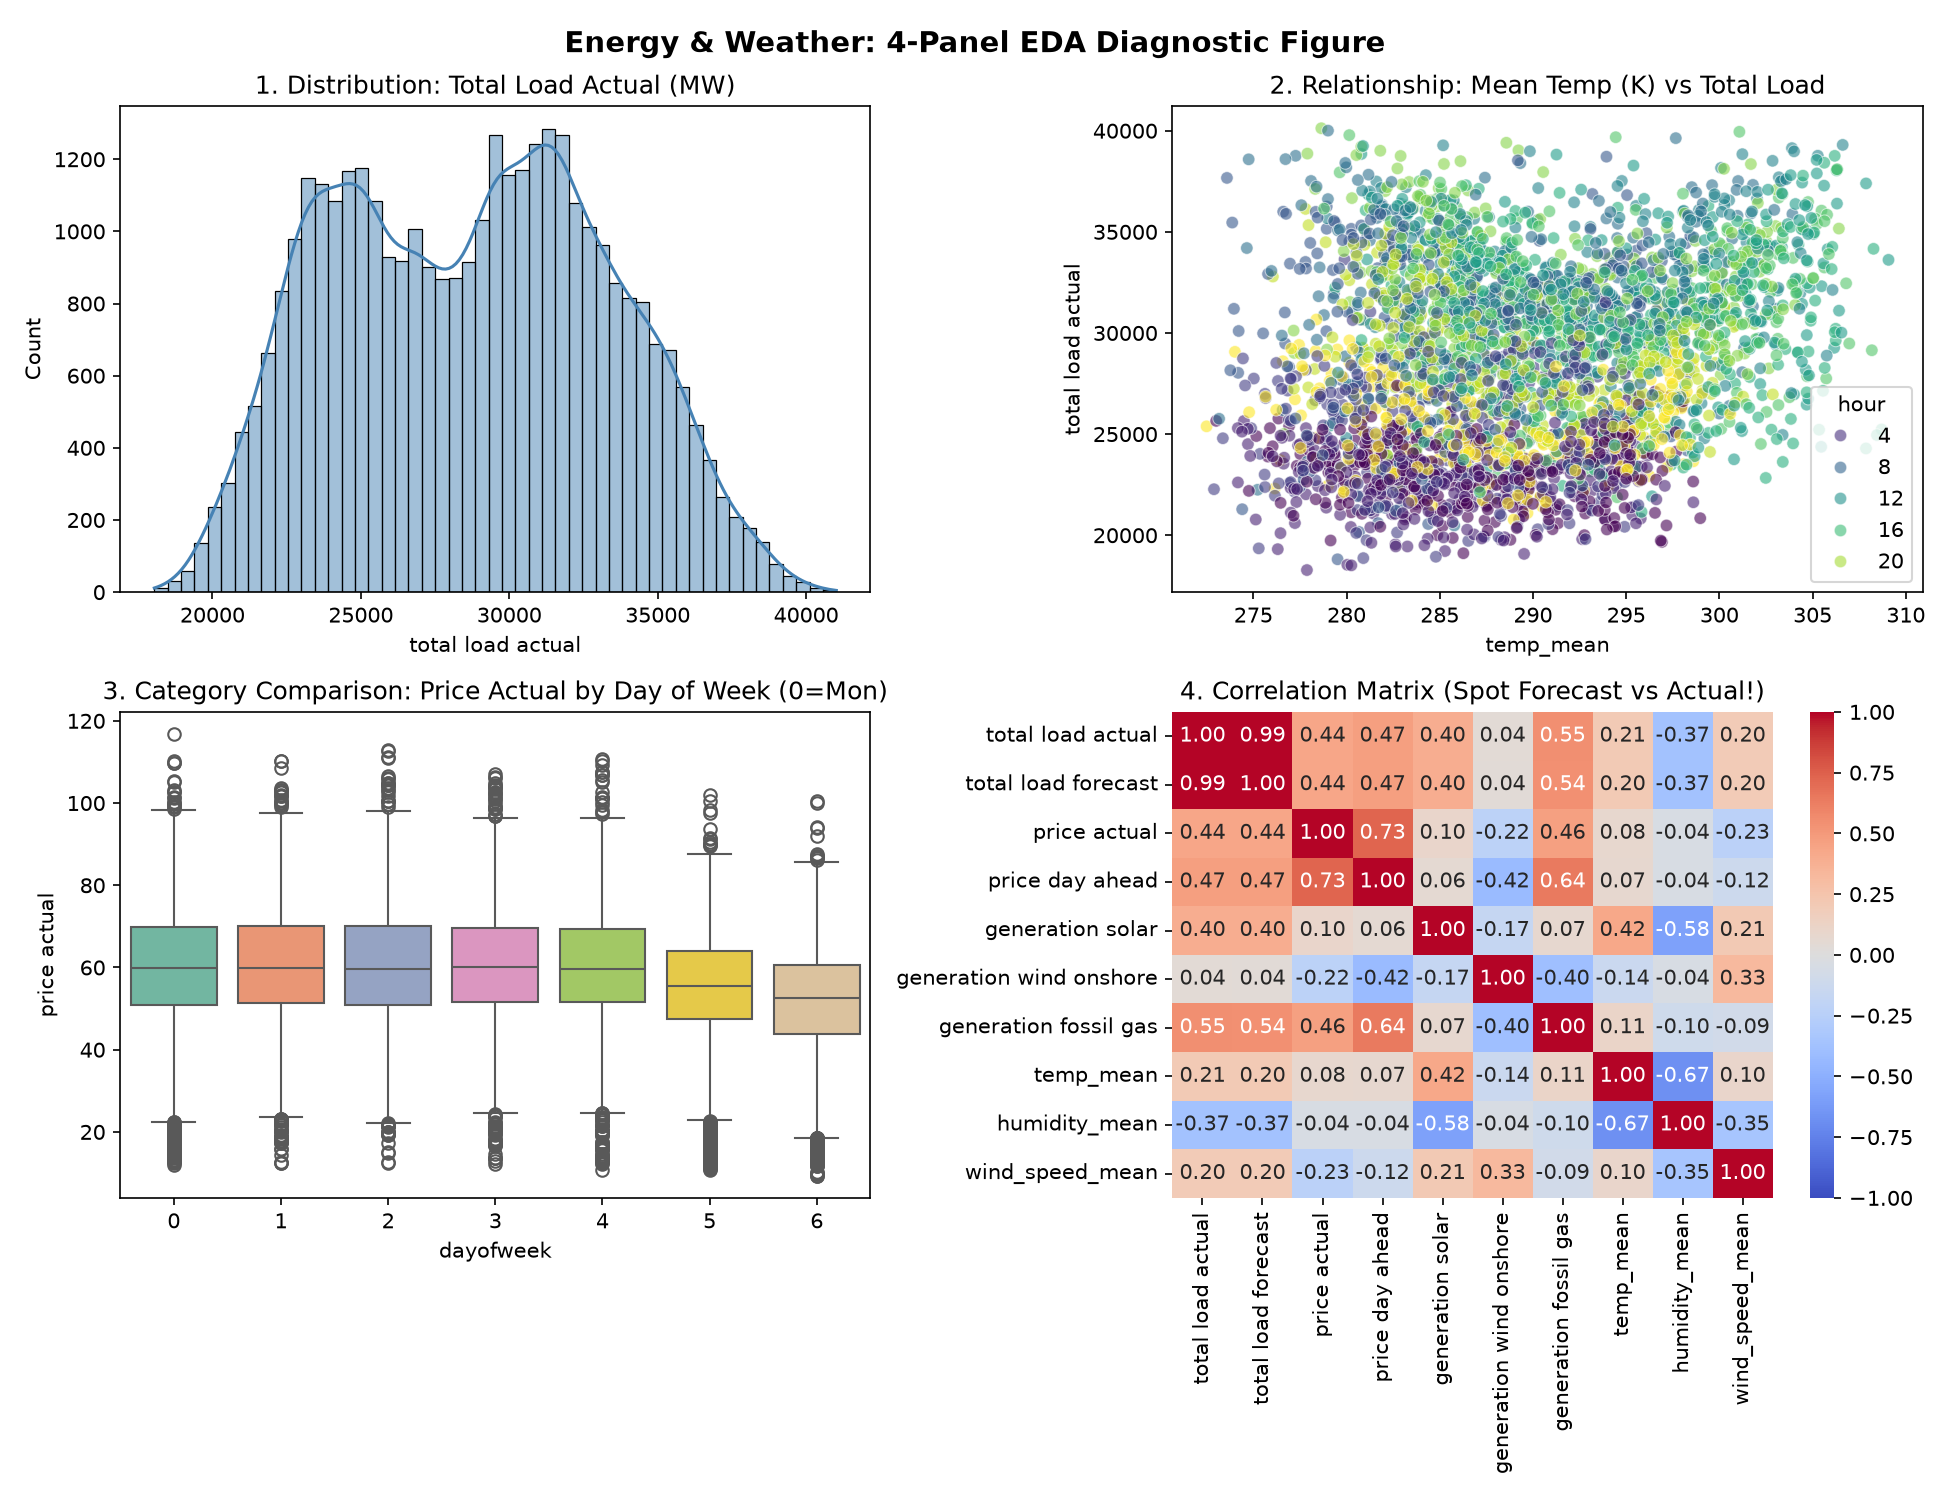
\includegraphics[width=0.92\linewidth]{eda_4panel.png}
\caption{Biểu đồ EDA 4 ô (phần A): phân phối phụ tải, quan hệ nhiệt độ--phụ tải, giá theo thứ, ma trận tương quan.}
\label{fig:eda}
\end{figure}

\todo{A viết chi tiết mục 3: mô tả cột, quy trình làm sạch, EDA, lý do chia theo thời gian.}
